\section{The p4est library}

Managing the mesh, especially when we have the presence of hanging nodes, is an important part of the work in any SEM implementation. This section thus present the library used, namely $p4est$ (the three dimensional equivalent is called $p8est$). 

The founding principles of $p4est$ are given in \cite{p4est}. In that article, they generate up to $5.13\: 10^{11}$ octants (the three dimensional equivalent of the quadrant) on as many as $2.2 \: 10^{5}$ CPU cores. Some additional information about the high-order node numbering can also be found in \cite{p4est2}. We present here only the features relevant to our work. 

We first present the approach to AMR used by $p4est$ and how it manages the dynamic refinement process, namely the refine and coarsen operators. We also explain the different structures used to build the mesh and the inherent terminology. 

In the second part, we will describe how, in our program, we handle hanging nodes leveraging $p4est$ and its structures. The way to compute the operator $R_{ij}^e$ (defined in the theory chapter) is also laid out. 

\subsection{AMR for p4est}

Different approaches exists for handling non conforming meshes. One strategy consists of splitting the computational domain into several unstructured macro-elements and then to refine them uniformly. The adaptivity is therefore only present at the coarse level. On the other hand, completely unstructured AMR yields more flexibility in the geometry but at a greater cost since there is no structure to rely on. Between the two are three-based methods, where each node is a quadrant that can have four children (which in turn can have children,...) or none at all. That recursive definition provides both simplicity and efficiency.

One downside is that the domain represented by a quadtree (a tree where a node is a leaf or has four children, as presented above) is always cube shaped. We can circumvent this problem by using a forest of quadtrees to represent a large range of geometrical shapes. 

The approach favored by $p4est$ is the latter : it handles the dynamic management of a collection of adaptive quadtrees, later called a forest of quadtrees. 

We can split the process used by $p4est$ in a two-level decomposition of the domain : first the definition of the forest, which we later call the macro-mesh, and then the adaptive recursive definition of each individual quadtree, later called the micro-mesh.

For the macro-mesh, the domain $\Omega \subset \mathbb{R}^2$ is split into $K$ conforming elements. Using $K$ conforming elements allows us to map more general domains than with a single quadtree since each corner of the macro-elements can be shared by more than 4 elements. There exists a mapping to each element from a reference element by a smooth function $\phi_k : [0;2^b]^2 \rightarrow \mathbb{R}^2$. Formally, we have that the domain $\Omega$ is split as : 

\begin{align*}
\Omega &= \bigcup_k \phi_k([0;2^b]^2) &0\leq k < K
\end{align*} 

We have an important thing to note here. It is an important feature of $p4est$ to perform all computations related to the connectivity and neighborhood relations discretely (i.e. it uses an integer-based approach). This is why the reference element is $[0;2^b]^2$. The main objective is to avoid floating-point arithmetic and the roundoff errors that might lead to errors in the topology. In their algorithms, the mappings $\phi_k$ are never used, except for the visualization and to encode the geometry that might be used for an external numerical application (such as ours). The consequence of having an integer-based system is that we cannot refine a quadtree indefinitely. Indeed, a quadrant cannot have a smaller length than 1 on the reference element. Thus, with $[0;2^b]^2$, it is possible to have at most $2^{2b}$ quadrants per element of the macro-mesh. Equivalently, each quadtree cannot have a depth superior to $b$, and a quadrant a refinement level superior to $b$. In the $p4est$ library, $b=29$, which yields a maximum of $2.9 \: 10^{17}$ quadrants per quadtree (the number would even be higher in three dimensions). We can see that it is amply sufficient for our applications. 

Let us also note that the macro-mesh cannot be changed dynamically and is shared among all processes. In practice, the number of quadtrees $K$ is thus limited by local memory. The experiments in \cite{p4est} go up to several million quadtrees.

Let us now turn to the micro-mesh. Based on a user-defined criterion, the refinement of the quadtree is often defined recursively. This creates a quadtree with the quadrants as leaves. Each quadrant of a given quadtree is then uniquely defined by the integer coordinates of its lower left corner $x,y \in \{0,1,2,...,2^b-1\}$ on the referent element and its level of refinement, i.e. the level of the leaf corresponding to that quadrant in the quadtree. In the reference element, a quadrant of level $l$ is a square of length $2^{b-l}$.


The details of the refine algorithm used in $p4est$ are not given here but can be found in \cite{p4est}. Here, non conforming edges are allowed. As mentioned in the theory chapter, our application only allows $1$-irregular meshes, i.e. two neighboring quadrants differ by at most one level of refinement. However, the refine function in $p4est$ does not constraint the size relations for neighboring quadrants (leading possibly to $k$-irregular meshes with $k>1$). Fortunately, the library also contains a balance function that we can use to guarantee a $1$-irregular mesh. Of course, the balance function acts both on quadrants in the same quadtree and on quadrants in different quadtrees that connect through an edge of the macro-mesh. 

The micro-mesh, i.e. the collection of quadrants, can be dynamically changed (with the refine and coarsen functions) and is shared between all processes. 

\begin{figure}
\centering
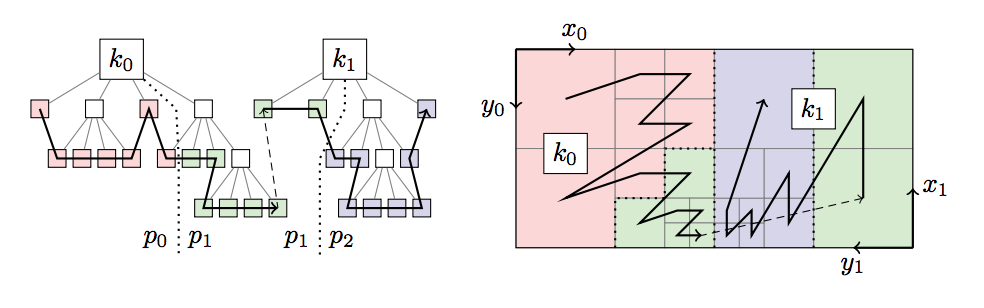
\includegraphics[scale=1.0]{Implementation/filling_curve.png}
\caption{One-to-one correspondence between a forest of quadtrees (left) and a computational domain (right). There are two quadtrees $k_0$ and $k_1$ (corresponding to two elements in the macro-mesh). Going through the leaves of the forest from left to right creates a space filling curve (in black) and thus a total ordering of the quadrants. Source : \cite{p4est}. }
\label{filling_curve}
\end{figure}

Tree-based AMR methods naturally lead to space filling curves. Indeed, if the global index of a quadrant is given by its order of appearance when looking at the forest of quatrees from left to right, then going quadrant by quadrant creates a curves that tends to fill the domain. An example of this is given in figure \ref{filling_curve}. On the left, we can see the forest which contains two quadtree ($k_0$ and $k_1$), distributed between three processes. We can also see that the refinement process has lead to quadrants with level 1, 2 and 3. On the right, the corresponding mesh is shown. Because we have different levels of refinement, the mesh is non conforming but it is still acceptable for our application since it is $1$-irregular. Inspecting the leaves in the forest of quadtrees from left to right creates a space filling curve that can be used to define a global index for the quadrants. We can see that, within one quadtree, the space filling curve follows the orientation of its coordinate axes.

There are still three things we want to point out in this part : how to tell if a quadrant is touching the boundary of the computational domain, how to obtain the physical coordinates of the corners of any quadrant and give some explanation about the global numbering of nodes used in the spectral elements method. 

\subsubsection{Quadrants on the boundary}

When we solve the system arising from SEM, it is fundamental to be able to tell whether a quadrant has one of its face on the boundary of the computational domain. 

Let us first note that if a quadrant has a face on the boundary, then the corresponding face of the macro-mesh element is on the boundary. 

In order to be able to tell about the neighboring quadtrees, there exists a function $k'=NO(k,f)$ that tells for a quadtree $k$ that its neighbor through face $f$ is $k'$, as well as a function $f' = NF(k,f)$ that tells that $k'$ is connected to $k$ through face $f'$. 

The convention used by $p4est$ to say that quadtree $k$ has face $f$ on the boundary is : 

\begin{align*}
NO(k,f) &= k\\
NF(k,f) &= f
\end{align*}

This convention only prevents the (pathological!) configuration where a quadtree connects to itself periodically through a face that is rotated against itself and that never happens in our application. That enables us to tell which quadrants have a face on the boundary. 

\subsubsection{Physical coordinates of the corners}

We are now looking at how to compute the physical coordinates of a quadrant. Let us first define the one dimensional linear mapping : 

\begin{align*}
\phi_0(x) &= 1-x\\
\phi_1(x) &= x
\end{align*}

Let us then assume that the quadrant is located in the macro-mesh element $k$. Let us also denote the physical coordinates of the corners of element $k$ by $x^k_i,y^k_i$ for $i=0,1,2,3$. Let us finally assume that the integer-based coordinate of the lower left corner of the quadrant are $x,y$ and it has a level of refinement $l$. In the reference element, the quadrant has therefore a length of :

$$ h = 2^{b-l} $$ 

Let us then use our linear mapping above to compute the coordinates of the corners of the quadrant $X_i,Y_i$ for $i=0,1,2,3$ as : 

\begin{align*}
X_{i+2j} &= \sum_{i=0}^1\sum_{j=0}^1 x^k_{i+2j} \phi_i(\frac{x+ih}{2^b})\phi_j(\frac{x+jh}{2^b}) &\text{for $i,j=0,1$}\\ 
Y_{i+2j} &= \sum_{i=0}^1\sum_{j=0}^1 y^k_{i+2j} \phi_i(\frac{x+ih}{2^b})\phi_j(\frac{x+jh}{2^b}) &\text{for $i,j=0,1$}\\ 
\end{align*}


Once we have the physical coordinates of any quadrants of our mesh, we can compute easily quantities such as the physical coordinates of the different local GLL nodes, the value of the jacobian,...

\subsubsection{Global unique node numbering}

Let us finally give some explanation about the globally unique numbering of the unknowns used in the spectral elements method. It is created in $p4est$ by a structure named $lnodes$. The principle is to number in order the global GLL nodes encountered while going through the quadrants by the global index. If there are no hanging nodes, it is simple : when we get to a quadrant, we number the nodes that have still not been numbered in lexicographic order then go to the next quadrant. When we have hanging nodes, it is more difficult since they are not independent and therefore cannot get a global numbering. The principle is then to number the global nodes that have an influence of the hanging nodes in the quadrant. 

\begin{figure}
\centering
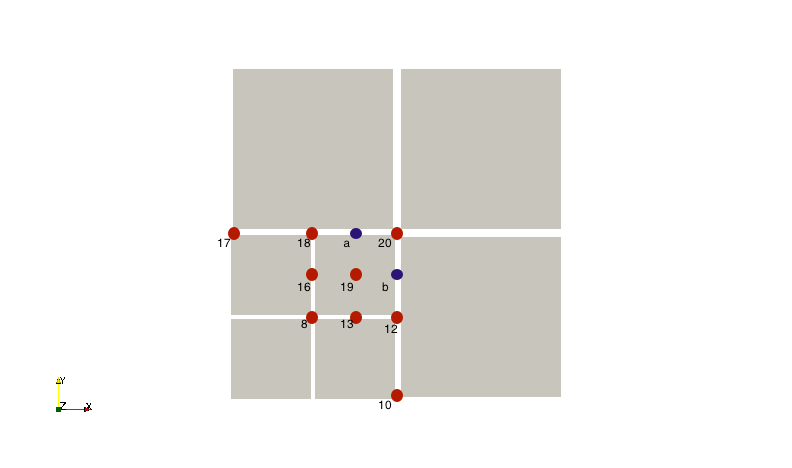
\includegraphics[scale=0.5]{Implementation/nodes_ex.png}
\caption{Global numbering of the nodes (in red) that have an influence in the small quadrant close to the center as well as the hanging nodes (in blue) for an interpolation of degree $p=2$. }
\label{nodes_ex}
\end{figure}

All this information is contained in a large array called $element\_nodes$ in $lnodes$. Let us give an example for the sake of clarity. Figure \ref{nodes_ex} shows a mesh for a degree of interpolation $p=2$ where we see in red the global nodes having an influence in the small quadrant close to the center. We can see that this quadrant has two hanging edges. The $element\_nodes$ array for this example is given by : 

$$element\_nodes = \begin{bmatrix}
8 &13& 10& 16 &19& 12 &17& 18& 20
\end{bmatrix}$$

We can see that it numbers the global GLL nodes first in the $x$ direction, then in the $y$ direction and uses the global numbering to refer to hanging nodes. It is possible to do this since hanging nodes are always located on edges. 

\subsection{Handling the hanging nodes}

Let us now look at how to practically handle hanging nodes. As presented before, the array $element\_nodes$ always uses global numbering to tell the nodes that have an influence in a quadrant. Therefore, we have to know which, if any, edges are hanging. This information, for each quadrant, is encoded in $face\_code$ in $lnodes$.

\subsubsection{Decoding the face code}

The function that we built to decode $face\_code$ returns $false$ if no edge is hanging while it returns $true$ and fill an array of length 4 called $hanging\_corner$ if there are at least one hanging edge where : 

\begin{align*}
hanging\_corner_i &= -1 &\text{if corner $i$ is not hanging}\\
&= a &\text{if $a$ is the non hanging corner corresponding to $i$}
\end{align*}

The $face\_code$ is a bitcode where the last two bits contain the position of the quadrant relative to its parent and the next two bits contain the status of the potentially hanging edges. Indeed, it is obvious that for any quadrant, at most two edges can be hanging. 

For example, in figure \ref{nodes_ex}, the $face\_code$ of the quadrant is $1111$ since it is the fourth child of its parent and the two potentially hanging nodes are indeed hanging. The $hanging\_corner$ array resulting from decoding that face code is : 

$$hanging\_corner = \begin{bmatrix}
-1 &3& 3& -1
\end{bmatrix}$$

Once we have the hanging corners, we can know which edges are hanging and if those edges constitute the first or the second part of the corresponding non hanging edge. For example in figure \ref{nodes_ex}, the east edge is hanging and constitute the second part of the corresponding non hanging edge defined by global nodes 10 and 20. 

\subsubsection{Computing $R_{ij}^e$}

All the information about the mesh computed above has two purposes : for us to be able to interpolate the different functions in each quadrant (scatter operation) and then to gather the result of the integration. As mentioned in the theory chapter, we never build the operator $R_{ij}^e$ explicitly. Let us first present the scatter operation. There are three positions possible for a local GLL node : 

\begin{enumerate}
\item The node is one of the four corners
\item The node is on an edge
\item The node is in the "interior", i.e. neither on an edge nor on a corner
\end{enumerate}

Let us stress the fact that only the first two types of nodes can be hanging. Therefore, the first step every time we need to perform an interpolation is to load the "interior", since we are sure those nodes are not hanging. In figure \ref{nodes_ex}, this corresponds to only one node (19).

The second step is to look at the edges. If an edge is not hanging, then we can load all nodes on this edge but the corners (since even on a non hanging edge, those can be hanging). In figure \ref{nodes_ex}, this corresponds to node 13 for the south edge and node 16 for the west edge. For the hanging edges, we need to perform an interpolation of the values at the global nodes to obtain the values at the hanging nodes. We can do a one dimensional interpolation since hanging nodes and the global nodes that influence them are located along an edge which is a straight line. In figure \ref{nodes_ex}, hanging nodes $b$ is interpolated using global nodes 10, 12 and 20.  Whether the hanging edge is the first or the second part of the non hanging edge is important since the interpolation will be different. Let us assume that the values at the global nodes are given by $u^{glob}_i$ for $i=0,...,p$. Then the value at hanging node $j$, $u^{loc}_j$, is given by : 

\begin{align*}
u^{loc}_j &= \sum_{k=0}^p l_k\left(\frac{\xi_j}{2}-\frac{1}{2}\right) u_k^{glob} &\text{if the hanging edge constitutes the first part}\\
u^{loc}_j &= \sum_{k=0}^p l_k\left(\frac{\xi_j}{2}+\frac{1}{2}\right) u_k^{glob} &\text{if the hanging edge constitutes the second part}
\end{align*}

Where $l_k$ denotes the Lagrangian polynomial associated with the $k$-th 1D GLL node. Since it is always the same interpolation (i.e. the coefficients of the linear combination do not depend on the quadrant) for all hanging edges, we built two matrices that perform the interpolation (one when the edge is the first part, $D^1$, and the other when the edge is the second part, $D^2$) and we use them every time we have a hanging edge. 

\begin{align*}
D^1_{ij} &= l_j\left(\frac{\xi_i}{2}-\frac{1}{2}\right)\\
D^2_{ij} &= l_j\left(\frac{\xi_i}{2}+\frac{1}{2}\right)
\end{align*}

For the example given in figure \ref{nodes_ex}, we have for the east edge :

$$ \begin{pmatrix}
u_{12} \\ u_b \\ u_{20}
\end{pmatrix} = \begin{pmatrix}
0 & 1 & 0\\
-0.125 & 0.75 & 0.375\\
0 & 0 & 1
\end{pmatrix}\begin{pmatrix}
u_{10} \\ u_{12} \\ u_{20}
\end{pmatrix}$$

Here we can also do the corners and mark them as visited.

The third step is to look at all four corners and check whether we have visited them or not. Those we have not yet visited are not hanging and we can therefore load them. In figure \ref{nodes_ex}, this corresponds to node 8. 

The gather operation works in much the same way. We first deal with the interior where we are sure no nodes are hanging. Then, we look at the edges. If the edge is hanging, we use the transpose of the matrices $D^1$ and $D^2$ to go from local nodes to global ones. We end with the corners that have not yet been visited. 


